\section{Технический проект}
\subsection{Общая характеристика организации решения задачи}

Необходимо спроектировать и разработать веб-приложение, направленное на поддержку самостоятельного изучения JavaScript иностранными студентами. Платформа представляет собой совокупность взаимосвязанных веб-сервисов, доступных через единый пользовательский интерфейс, реализованный с использованием современных веб-технологий: HTML, CSS, JavaScript и Python (Django).

Каждый сервис (модуль) обеспечивает выполнение образовательных задач: управление курсами, уроками, тестами, результатами и локализацией. Платформа размещается в сети Интернет по определённому доменному имени (например, https://swsueducate.ru). Интерфейс реализован с использованием фреймворка Bootstrap для адаптивности, а клиентская интерактивность обеспечивается через JavaScript (например, Sortable.js для сортировки уроков). Серверная часть, построенная на Django, обрабатывает запросы, управляет данными и генерирует динамические страницы.

\subsection{Обоснование выбора технологии проектирования}

На сегодняшний день информационный рынок, поставляющий программные решения в выбранной сфере, предлагает множество продуктов, позволяющих достигнуть поставленной цели – разработки веб-платформы.

\subsubsection{Описание используемых технологий и языков программирования}

В процессе разработки веб-платформы используются программные средства и языки программирования. Каждое программное средство и каждый язык программирования применяется для круга задач, при решении которых они необходимы.

\subsubsection{Язык программирования Python}

Python — это высокоуровневый язык программирования общего назначения с поддержкой нескольких парадигм, включая объектно-ориентированное, процедурное и функциональное программирование. Благодаря своей простоте, читаемости и обширной экосистеме библиотек, Python широко применяется в разработке веб-приложений, автоматизации процессов, анализе данных, машинном обучении и многих других областях. В контексте разработки веб-приложений Python используется совместно с фреймворками, такими как Django и Flask, которые обеспечивают удобные средства для создания серверной логики, обработки запросов и генерации динамических веб-страниц.

\subsubsection{Язык программирования JavaScript}

\paragraph{Достоинства языка JavaScript}

JavaScript — это высокоуровневый интерпретируемый язык программирования, основной задачей которого является создание интерактивного поведения на веб-страницах. Он является неотъемлемой частью технологии разработки клиентской части веб-приложений и поддерживается всеми современными веб-браузерами. С помощью JavaScript можно реализовывать динамическое обновление содержимого, проверку данных на стороне клиента, обработку событий, а также взаимодействие с сервером без перезагрузки страницы (через AJAX-запросы). Современные стандарты JavaScript (начиная с ECMAScript 6) предоставляют широкий набор возможностей, включая модули, асинхронные функции, классы и работу с промисами. Для повышения совместимости и ускорения разработки часто используются библиотеки и фреймворки, такие как jQuery, React, Vue.js и другие. Они позволяют упростить доступ к элементам DOM, реализовать реактивные интерфейсы и обеспечить кроссбраузерную поддержку. JavaScript выполняется непосредственно в браузере пользователя, что позволяет создавать отзывчивые и интерактивные пользовательские интерфейсы без необходимости постоянной связи с сервером.

\paragraph{Недостатки языка JavaScript}

\begin{itemize}
  \item parseInt("08") // → 0
  \item parseInt("0x10") // → 16
  \item parseInt("0x10", 10) // → 0
  \item null == 0 // → false
  \item null > 0 // → false
  \item null >= 0 // → true
  \item undefined == null // → true
  \item undefined === null // → false
  \item typeof NaN // → "number"
  \item NaN === NaN // → false
  \item "5" + 3 // → "53"
  \item "5" - 3 // → 2
  \item "5" * "3" // → 15
  \item "5" * "abc" // → NaN
  \item 0.1 + 0.2 === 0.3 // → false
  \item (0.1 + 0.2).toFixed(1) // → "0.3"
  \item true + true // → 2
  \item true - false // → 1
  \item "1" + true // → "1true"
  \item "1" - true // → 0
\end{itemize}



\subsection{Диаграмма компонентов и схема обмена данными между сервисами}

Диаграмма компонентов отображает взаимодействие пользователей (студентов и преподавателей) с сервисами платформы. Она помогает определить архитектуру, показывая связи между компонентами, включая клиентскую часть и серверную часть. Основными элементами диаграммы являются компоненты (например, курсы), их интерфейсы и зависимости между ними.

\begin{figure}[ht]
\center{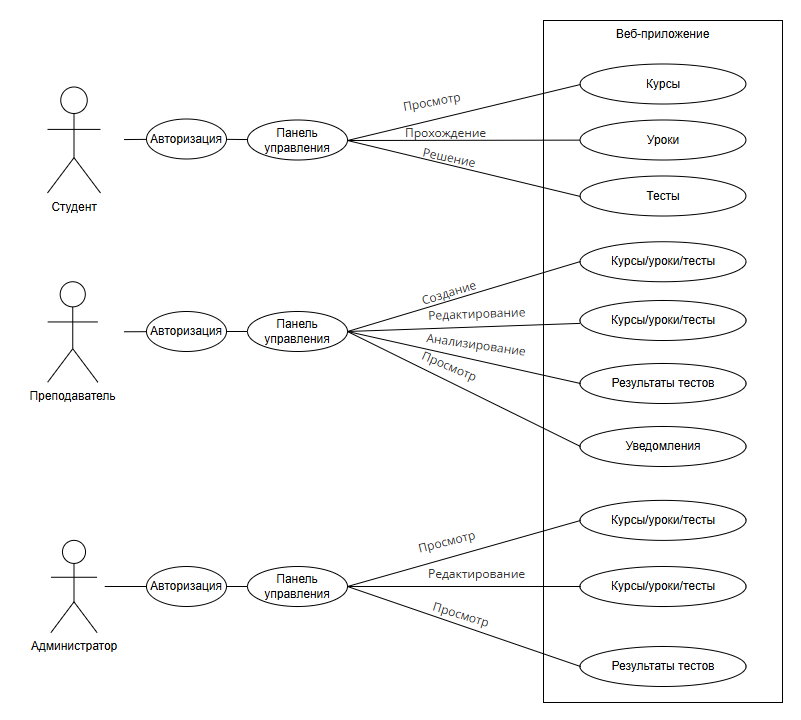
\includegraphics[width=1\linewidth]{images/UML}}
\caption{Диаграмма компонентов}
\label{comp:image}
\end{figure}

После авторизации в веб-платформе пользователь переходит на главную рабочую страницу <<панель управления для преподавателей или список курсов для студентов>>,  где отображаются доступные модули.

\begin{itemize}
    \item Сервис <<Курсы>> — позволяет преподавателям создавать, редактировать и удалять курсы, а студентам --- просматривать доступные курсы и записываться на них. В сервисе отображается список курсов с кратким описанием и статусом (например, доступен или завершён).
    
    \item Сервис <<Уроки>> — предоставляет преподавателям возможность добавлять, редактировать и сортировать уроки в рамках курса. Студенты могут изучать материалы уроков (текст, изображения, видео). Сервис поддерживает предпросмотр уроков для преподавателей.

    \item Сервис <<Тесты>> — позволяет преподавателям создавать тесты с вопросами и вариантами ответов. Студенты проходят тесты, получая автоматическую оценку. Сервис интегрирован с модулем результатов для отслеживания успеваемости.

    \item Сервис <<Результаты тестов>> — предоставляет преподавателям инструменты для просмотра, анализа и удаления результатов тестов. Студенты могут видеть свои баллы и статистику по попыткам.

    \item Сервис <<Локализация>> — позволяет пользователям переключать язык интерфейса (например, русский, английский), что упрощает использование платформы для иностранных студентов. Поддерживается через Django-теги.

    \item Сервис <<Уведомления>> — отображает сообщения об успешных действиях (например, добавление урока, удаление результатов) или ошибках.

    \item Сервис <<Панель управления>> — главная страница для преподавателей, содержащая виджеты для быстрого доступа к курсам, урокам, тестам и результатам. Для студентов отображается список доступных курсов.

\end{itemize}

\subsection{Диаграмма размещения}

Диаграмма размещения (рис.~\ref{system:image}) отражает физические взаимосвязи между программными и аппаратными компонентами системы.

\clearpage
\begin{figure}[htp!]
	\centering{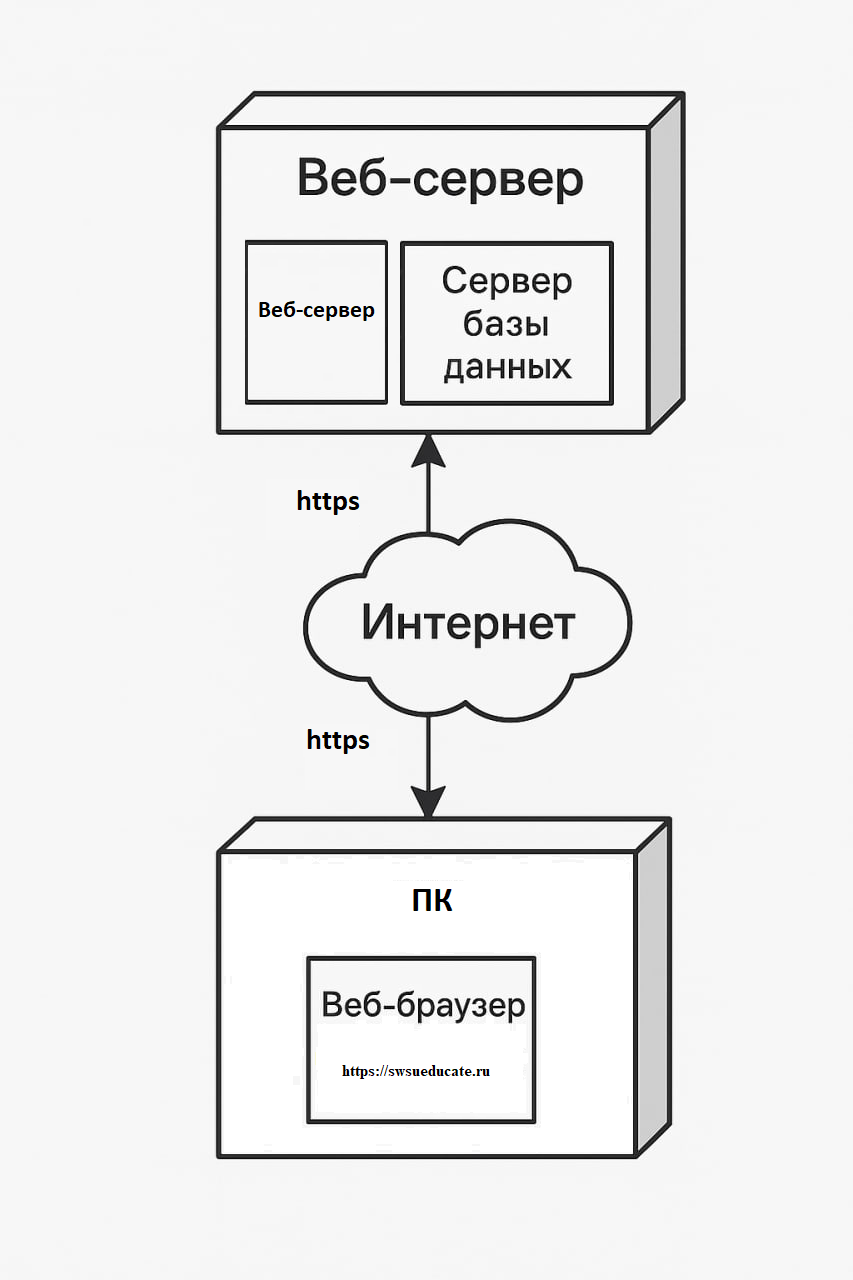
\includegraphics[width=0.5\linewidth]{images/диаграмма2}}
	\caption{Диаграмма размещения}
	\label{system:image}
\end{figure}


\subsection{Содержание информационных блоков. Основные сущности}

Проанализировав требования, можно выделить следующие основные сущности:

\begin{itemize}
  \item "<Курсы">;
  \item "<Уроки">;
  \item "<Тесты">;
  \item "<Результаты тестов">;
  \item "<Пользователи">;
  \item "<Локализация">;
  \item "<Уведомления">;
  \item "<Панель управления">.
\end{itemize}

В состав сущностей входят следующие атрибуты:

\begin{xltabular}{\textwidth}{|l|l|p{3.2cm}|X|}
  \caption{Атрибуты сущности <<Курсы>>\label{courses:table}}\\ \hline
  Поле & Тип & Обязательное & Описание \\ \hline
  \endfirsthead
  \continuecaption{Продолжение таблицы \ref{courses:table}}\\ \hline
  Поле & Тип & Обязательное & Описание \\ \hline
  \endhead
  id & Integer & true & Уникальный идентификатор курса \\ \hline
  title & String & true & Название курса \\ \hline
  description & Text & false & Описание курса \\ \hline
  teacher & ForeignKey & true & Преподаватель (ссылка на пользователя) \\ \hline
  createdAt & DateTime & true & Дата создания \\ \hline
\end{xltabular}

\begin{xltabular}{\textwidth}{|l|l|p{3.2cm}|X|}
  \caption{Атрибуты сущности <<Уроки>>\label{lessons:table}}\\ \hline
  Поле & Тип & Обязательное & Описание \\ \hline
  \endfirsthead
  \continuecaption{Продолжение таблицы \ref{lessons:table}}\\ \hline
  Поле & Тип & Обязательное & Описание \\ \hline
  \endhead
  id & Integer & true & Уникальный идентификатор урока \\ \hline
  course & ForeignKey & true & Курс, к которому относится урок \\ \hline
  title & String & true & Название урока \\ \hline
  content & Text & false & Содержимое урока (текст, HTML) \\ \hline
  order & Integer & true & Порядок урока в курсе \\ \hline
  createdAt & DateTime & true & Дата создания \\ \hline
\end{xltabular}

\begin{xltabular}{\textwidth}{|l|l|p{3.2cm}|X|}
  \caption{Атрибуты сущности <<Тесты>>\label{tests:table}}\\ \hline
  Поле & Тип & Обязательное & Описание \\ \hline
  \endfirsthead
  \continuecaption{Продолжение таблицы \ref{tests:table}}\\ \hline
  Поле & Тип & Обязательное & Описание \\ \hline
  \endhead
  id & Integer & true & Уникальный идентификатор теста \\ \hline
  lesson & ForeignKey & true & Урок, к которому относится тест \\ \hline
  title & String & true & Название теста \\ \hline
  questions & Array & false & Список вопросов (JSON или связанные модели) \\ \hline
  createdAt & DateTime & true & Дата создания \\ \hline
\end{xltabular}

\begin{xltabular}{\textwidth}{|l|l|p{3.2cm}|X|}
  \caption{Атрибуты сущности <<Результаты тестов>>\label{test_results:table}}\\ \hline
  Поле & Тип & Обязательное & Описание \\ \hline
  \endfirsthead
  \continuecaption{Продолжение таблицы \ref{test_results:table}}\\ \hline
  Поле & Тип & Обязательное & Описание \\ \hline
  \endhead
  id & Integer & true & Уникальный идентификатор результата \\ \hline
  student & ForeignKey & true & Студент (ссылка на пользователя) \\ \hline
  lesson & ForeignKey & true & Урок, связанный с тестом \\ \hline
  score & Integer & true & Оценка (в процентах) \\ \hline
  attempts & Integer & true & Количество попыток \\ \hline
  completedAt & DateTime & true & Дата завершения \\ \hline
\end{xltabular}

\begin{xltabular}{\textwidth}{|l|l|p{3.2cm}|X|}
  \caption{Атрибуты сущности <<Пользователи>>\label{users:table}}\\ \hline
  Поле & Тип & Обязательное & Описание \\ \hline
  \endfirsthead
  \continuecaption{Продолжение таблицы \ref{users:table}}\\ \hline
  Поле & Тип & Обязательное & Описание \\ \hline
  \endhead
  id & Integer & true & Уникальный идентификатор пользователя \\ \hline
  username & String & true & Имя пользователя \\ \hline
  email & String & true & Электронная почта \\ \hline
  isteacher & Boolean & true & Признак преподавателя \\ \hline
  avatar & String & false & Путь к аватару \\ \hline
  language & String & false & Предпочитаемый язык интерфейса \\ \hline
\end{xltabular}

\begin{xltabular}{\textwidth}{|l|l|p{3.2cm}|X|}
  \caption{Атрибуты сущности <<Локализация>>\label{localization:table}}\\ \hline
  Поле & Тип & Обязательное & Описание \\ \hline
  \endfirsthead
  \continuecaption{Продолжение таблицы \ref{localization:table}}\\ \hline
  Поле & Тип & Обязательное & Описание \\ \hline
  \endhead
  id & Integer & true & Уникальный идентификатор перевода \\ \hline
  key & String & true & Ключ перевода (например, "Delete") \\ \hline
  language & String & true & Язык (например, "ru", "en") \\ \hline
  value & String & true & Переведённый текст \\ \hline
\end{xltabular}

\begin{xltabular}{\textwidth}{|l|l|p{3.2cm}|X|}
  \caption{Атрибуты сущности <<Уведомления>>\label{notifications:table}}\\ \hline
  Поле & Тип & Обязательное & Описание \\ \hline
  \endfirsthead
  \continuecaption{Продолжение таблицы \ref{notifications:table}}\\ \hline
  Поле & Тип & Обязательное & Описание \\ \hline
  \endhead
  id & Integer & true & Уникальный идентификатор уведомления \\ \hline
  user & ForeignKey & true & Пользователь, получивший уведомление \\ \hline
  message & String & true & Текст уведомления \\ \hline
  type & String & true & Тип (успех, ошибка, предупреждение) \\ \hline
  createdAt & DateTime & true & Дата создания \\ \hline
\end{xltabular}

\begin{xltabular}{\textwidth}{|l|l|p{3.2cm}|X|}
  \caption{Атрибуты сущности <<Панель управления>>\label{dashboard:table}}\\ \hline
  Поле & Тип & Обязательное & Описание \\ \hline
  \endfirsthead
  \continuecaption{Продолжение таблицы \ref{dashboard:table}}\\ \hline
  Поле & Тип & Обязательное & Описание \\ \hline
  \endhead
  id & Integer & true & Идентификатор виджета \\ \hline
  name & String & true & Название виджета \\ \hline
  type & String & true & Тип виджета (список курсов, статистика) \\ \hline
  datasource & String & true & Источник данных (например, URL) \\ \hline
\end{xltabular}


Экземпляры этих сущностей реализуются в информационных блоках пользовательского интерфейса. Атрибуты сущностей отображаются в полях, свойствах и компонентах соответствующих элементов.
